\documentclass[a4paper, 12pt]{article}
\usepackage{geometry} 
\geometry{letterpaper, margin=1in}
\usepackage{amsmath}
\usepackage{amssymb}  
\usepackage{amsthm}
\usepackage{ulem} 
\usepackage{graphicx}
\usepackage{enumitem} % use for making lettered list 
\usepackage{bbm} % use for making the 1 identity operator EX: \mathbbm{1}
\usepackage{subfig}
\usepackage{indentfirst}
\usepackage{url}
\usepackage{setspace}
\doublespace
\graphicspath{ {images/} }

% format to allow bolded theorems, corollaries, etc... 
\newtheorem*{theorem}{Theorem}
\newtheorem*{corollary}{Corollary}
\newtheorem*{lemma}{Lemma}
\newtheorem*{Example}{Example} 
\newtheorem*{Remark}{Remark}
\newcommand{\definition}[1]{
  \begin{minipage}[c]{0.85\textwidth}
    \vspace{2 em}
    \textbf{Definition:} \textit{#1}
    \vspace{2 em}
  \end{minipage}
}



% stop typing \mathbb a thousand times 
\newcommand{\R}{\mathbb{R}}
\newcommand{\C}{\mathbb{C}}
\newcommand{\F}{\mathbb{F}}
\newcommand{\Mat}[2]{\mathcal{M}_{#1\times#2}}

% change margins for solution
\newenvironment{solution}{%
	\begin{list}{}{%
			\setlength{\topsep}{0pt}%
			\setlength{\leftmargin}{1.5cm}%
			\setlength{\rightmargin}{1.5cm}%
			\setlength{\listparindent}{\parindent}%
			\setlength{\itemindent}{\parindent}%
			\setlength{\parsep}{\parskip}%
		}%
		\item[]}{\end{list}}

\title{Distance Functions and the Images of Some Common Figures}
\date{\today}
\author{John Waczak\\MTH 338 \hspace{1em} Dr. Ren Guo} 
\begin{document}
\maketitle


\section*{Background}

In class we have discussed models for many different geometries. In our discussion, we employed the Kleinian view of geometry \cite{brannan}, that is:

\definition{A \textbf{Geometry} is a set of points called the \textit{space} along with a group of transformations which act upon the space. }

\noindent From this definition we decided that to study geometry is to study the properties of figures that are unchanged by these transformations. The first three geometries we considered-- Euclidean, affine, and projective, all involved the standard Euclidean space of $\R^n$. For affine geometry we considered transformations of figures in the plane ($\R^2$) as a model for the process of \textit{parallel projection}. Similarly, in projective geometry, the space of consideration was $\R^3$ which we used to make precise the artistic concept of perspective.

For each of these geometries we developed a list of preserved properties. As an example, for affine geometry, this included properties such as
\begin{itemize}
\item Straight lines map to straight lines
\item Parallel lines map to parallel lines 
\item Ratios of lengths are preserved
\end{itemize}

The final property listed above is not true for projective geometry where instead only the cross-ratio is preserved. Therefore, we can see that having a notion of distance is valuable so that one may test what kinds of properties the transformation group of a geometry does preserve. Furthermore, defining a distance function enables the use of coordinates to perform direct calculations-- a process that can simplify many proofs. This paper will explore distance functions and the images of figures under them.  

\section*{Euclidean Distance}
Perhaps the most familiar of geometries, Euclidean geometry studies the space $\R^n$ (for us $\R^2$) and the properties that remain unchanged under the isometry group of transformations. Isometries are transformations that preserve distance and thus, members of this group are of the form
\begin{equation*}
  t(\mathbf{x}) = \mathbf{U}\mathbf{x} + \mathbf{a}
\end{equation*}
where $\mathbf{U}$ is an orthogonal $n\times n$ matrix and $\mathbf{a}$ is a vector in $\R^n$ \cite{brannan}. This means that Euclidean transformations involve rotation, reflection, and translation (or compositions thereof).

In this space, the \textbf{Euclidean distance function} is defined as
\begin{equation*}
  d(x,y) = \left( \sum\limits_i^n |x_i-y_i|^2\right)^{\frac{1}{2}}
\end{equation*}
for points $x,y\in\R^n$ which comes from the famous \textit{Pythagorean Theorem}. This distance function is rightly called the straight line distance as it computes the length of the straight line that passes through the points x and y.
\begin{figure}[!hbt]
  \centering
  \includegraphics[width=0.4\textwidth]{EuclideanDistance}
  \caption{Illustration of the Euclidean distance $d$ between two points $(x_1,y_1)$ and $(x_2, y_2)$. }
  \label{fig:EuclideanDistance}
\end{figure}

In it's simplest form, $x,y$ each have one component and therefore the Euclidean distance reduces to
\begin{equation*}
  d(x,y) = \sqrt{|x-y|^2} = |x-y|
\end{equation*}

Using this definition of distance, it is easy to prove many simple properties of geometries on Euclidean spaces. The following is one such example taken from affine geometry.
\begin{theorem}[Ceva's Theorem]
  Let $\Delta ABC$ be a triangle and let X be a point which does not lie on any of its (extended) sides. If AX meets BC at point P, BX meets CA at point Q, and CX meets BA at point R, then
  \begin{equation*}
    \frac{AR}{RB}\cdot\frac{BP}{PC}\cdot\frac{CQ}{QA} = 1
  \end{equation*}
  \begin{figure}[!hbt]
    \centering
    \includegraphics[width=0.5\textwidth]{CevasTheorem}
    \caption{Triangle illustrating Ceva's theorem. Taken from \cite{brannan}}
    \label{fig:Ceva}
  \end{figure}
\end{theorem}

To prove this theorem, one can construct the coordinates of such a triangle and then use the fundamental theorem of affine geometry to map the triangle and the point X to the standard triangle with $A'=(0,1)$, $B'=(0,0)$, $C'=(1,0)$, and $X'=(u,v)$ for some $u,v\in\R$. Having the distance function then enables the direct calculation of the distances involved in the ratios.

\section*{Hyperbolic Distance}
In hyperbolic geometry, we consider instead the points of $\mathcal{D}$, the Poincare disk that is defined as
\begin{equation*}
  \mathcal{D} = \{ z\in\C : d(z,\mathcal{O})<1\}
\end{equation*}
where $\mathcal{O}$ is the origin. In this space, we define the hyperbolic distance to be
\begin{equation*}
  d_H(z_1, z_2) = \tanh^{-1}\left(\left|\frac{z_2-z_1}{1-\overline{z_1}z_2} \right|\right)
\end{equation*}
Clearly, this equation is very different from the Euclidean distance function and we can expect that this leads to some interesting properties for hyperbolic geometry. Consider the hyperbolic distance between the points $z_1 = 0.1$ and $z_2 = 0.5$ along the real axis of $\mathcal{D}$. Their distance is
\begin{align*}
  d_H(z_1, z_2) &= d_H(0.1, 0.5) \\
  &= \tanh^{-1}\left(\left| \frac{0.5-0.1}{1-0.1\cdot0.5}\right|\right)\\
  &= \tanh^{-1}\left(\left| \frac{0.4}{0.95}   \right|\right)\\
  &\approx 0.449
\end{align*}
This is value is more than $10\%$ larger than the Euclidean distance of 0.4-- not what you would expect when using the Euclidean distance. In fact, as a point moves closer to the edge of $\mathcal{D}$, its distance from the origin tends to infinity.  
\section*{The Distance Function}
Both $d$ and $d_H$ are examples of distance functions for two different spaces but what is a distance function? In theory, a distance function should take two points in a space a return back a number in such a way as to allow a meaningful comparison of the two points. This boils down to the following requirements

\definition{A \textbf{distance function} or metric on a space V, is a function $d:V\to \R$ satisfying the following conditions
  \begin{enumerate}
  \item $d(x,y)\geq 0$ $\forall x,y \in V$  
  \item $d(x,y) = 0$ if and only if $x=y$
  \item $d(x,y) = d(y,x)$
  \item $d(x,z) \leq d(x,y) + d(y,z)$
  \end{enumerate}
}

As an exercise, let's verify that the Euclidean distance function $d$ satisfies these properties.
\begin{solution}
  \noindent(pf.) The first two requirements are easily verified by inspection of the distance function. We have that
  \begin{equation*}
    d(x,y) = \left(\sum_i^n |x_i-y_i|^2\right)^{\frac{1}{2}}
  \end{equation*}
  therefore, we certainly have $d\geq 0$ as the summand is nonnegative due to the absolute value and the squaring. We can also see that $d=0$ if and only if $x_i =y_i$ $\forall i$ i.e. $x=y$. The third condition is also satisfied by $d$ as swapping $x,y$ has no effect, again due to the absolute value and squaring. Finally, for the fourth condition, recall that by for two vectors $x,z$ in $\R^n$ we have
  \begin{equation*}
    d(x,z) = ||x-z|| = (x-z)\cdot(x-z)
  \end{equation*}
  where $\cdot$ is the standard vector dot product. Also recall that the Cauchy-Schwarz inequality gives
  \begin{equation*}
    x\cdot z \leq ||x||\;||z||
  \end{equation*}
  then for a third vector $y\in\R^n$ consider the following
  \begin{align*}
    ||x+y||^2 &= (x+y)\cdot(x+y) = ||x||^2+2(x\cdot y) + ||y||^2 \\
    &\leq ||x||^2+2||x||\;||y|| + ||y||^2 \\
    &= \left(||x||+||y||\right)^2 \\
    \Rightarrow ||x+y|| &\leq ||x|| + ||y|| 
  \end{align*}
  Now, using this new fact, we can re-write the $d(x,z)$ equation.
  \begin{align*}
    d(x,z) &= ||x-z|| \\
    &= ||x-z+y-y|| \\
    &= ||(x-y) + (y-z)|| \\
    &\leq ||x-y|| + ||y-z|| \\
    &= d(x,y) + d(z,y) 
  \end{align*}
    Therefore we see that the Euclidean distance function does indeed satisfy all four properties.\qed
\end{solution}

It is slightly more challenging to show that the hyperbolic distance $d_h$ also satisfies these requirements. For a reasonable derivation, consult section 3 of chapter 6 in \cite{brannan}.  

There are many other distance functions to consider. First, we can imagine generalizing the Euclidean distance function $d$. All of the properties we needed for $d$ to be a true distance function are satisfied by the inner most $|x_i-y_i|$ calculation. Thus, let $p\in\mathbb{N}$ and consider the function
\begin{equation*}
  d_p(x,y) = \left(\sum_i^n|x_i-y_i|^p\right)^{\frac{1}{p}}
\end{equation*}
We will call this the generalized Euclidean distance. Next, let's instead go the other direction. Consider the simpler equation given by
\begin{equation*}
  d_\text{taxi}(x,y) = \sum_i^n |x_i-y_i|
\end{equation*}
This distance function is called the taxicab or Manhattan metric. It arises if we consider a grid of points akin to the blocks of a major city. If a car wanted to move from point x to point y, it could not travel in a straight line and so the distance traveled is truly the sum of the horizontal and vertical distances traveled.

Finally, we might also decide that we only care to consider the largest of either the horizontal or vertical displacements. This leads to the sup norm (for suprememum) and is defined as
\begin{equation*}
  d_\text{sup} = \max\{|x_i-y_i|\}
\end{equation*}

\section*{Circles}
Now that we have defined many different distance functions a natural question is what do the images of particular curves look like under these functions. Recall from class that the definition of a circle is
\begin{equation*}
  \mathcal{C} = \{p \;\; | \;\;d(p,\mathcal{O})=r\}
\end{equation*}
that is, a circle is defined as the set of all points p which have a constant distance $r$ to some center $\mathcal{O}$. Because this figure is nicely defined for us in term of distances, we can explore the unit circle of each of our distance functions in order to examine how they are related. Let's begin with the p=1 distance function, i.e. the taxicab metric.

It is easy to consider first the edge cases. We have that $d(x,y) = \sum_i^n|x_i-y_i|$. Here we let the point $x=(0,0)$ be the origin so that each point p on the unit circle is given by $d(0,p)=\sum_i^n|p_i|=1$. Certainly, we have that the points $(1,0)$, $(-1,0)$, $(0,1)$, $(0,-1)$ all have distance 1. As the coordinates of the point p vary, we then expect to move between these four corners. Because our distance is just the sum of the magnitude of the coordinates, the unit circle connects these corners by straight lines.

For our generalized Euclidean distance, if we let $p=2$ we get the comfortable straight line distance function. Under this formula, the unit circle appears as the standard uniformly round figure. This image changes as we let p increase resulting in a squashing of the image. If we consider the sup metric, then our unit circle is formed by only considering the maximum of the two coordinates of a point. This results in a square circle *chuckle*. The following figure shows a plot of the unit circle under a variety of these distance functions.

\begin{figure}[!hbt]
  \hspace{-9em}
  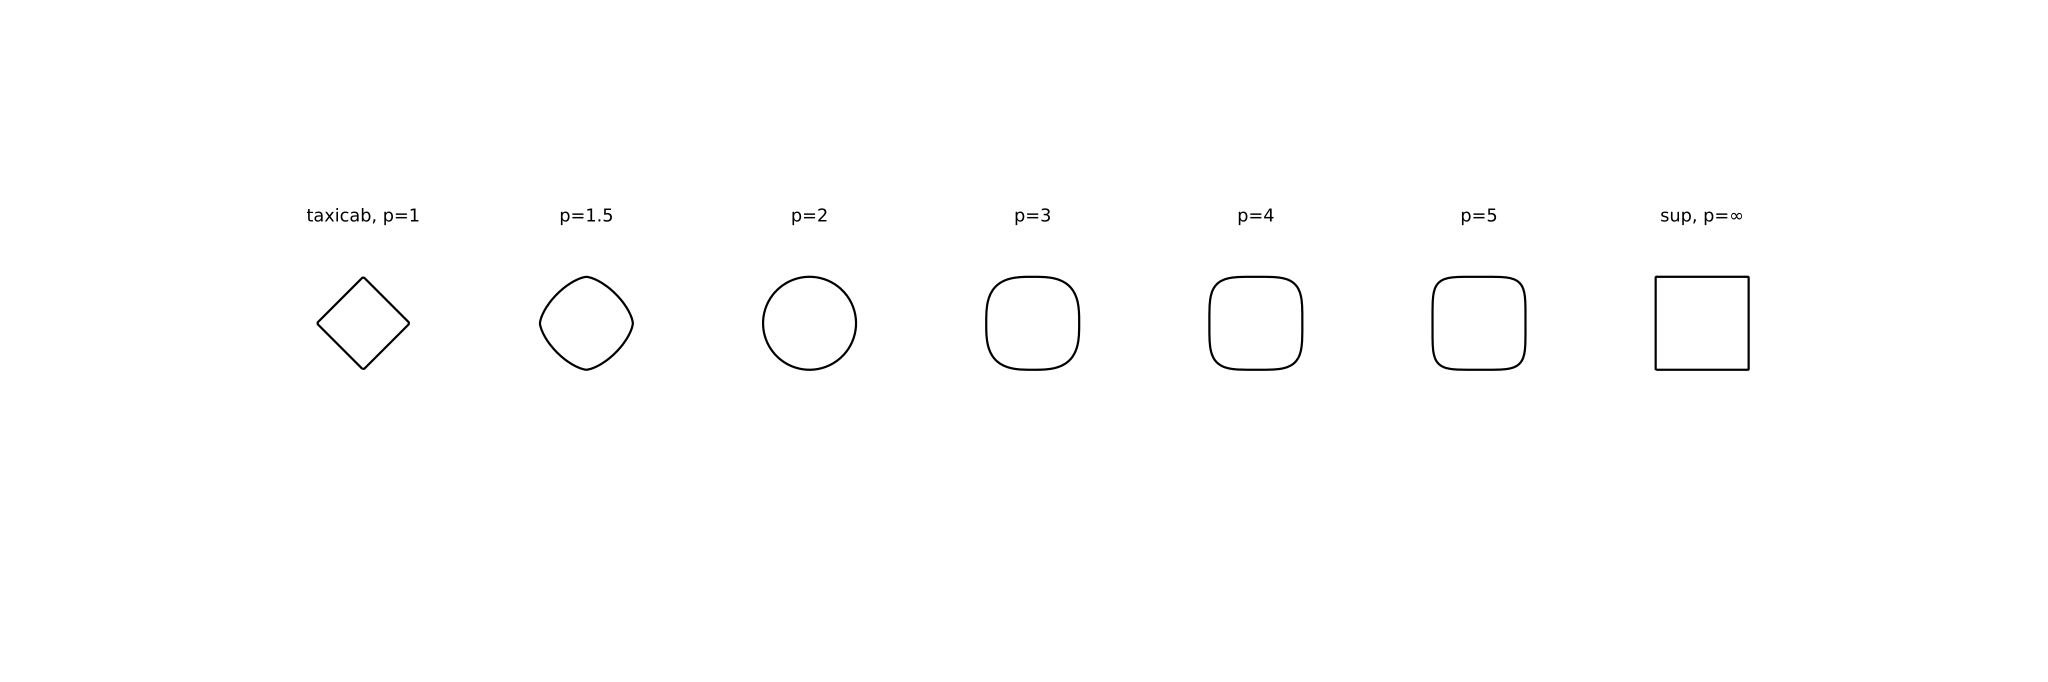
\includegraphics[width=1.4\textwidth]{unitCircles}
  \caption{The unit circle for various distance functions}
  \label{fig:unitCircles}
\end{figure}

From figure \ref{fig:unitCircles}, we can actually make some interesting observations. Starting at $p=2$, the standard Euclidean distance function we see that as $p$ increases, the image of the unit circle tends more to a square. In fact, I labeled the final unit circle for the sup distance with $p=\infty$ anticipating the following conjecture:
  \begin{equation*}
    \lim_{p\to\infty}\left(\sum_i^n|x_i-y_i|^p\right)^{\frac{1}{p}} = \max\left\{|x_i-y_i|\right\}
  \end{equation*}

 To show the equality holds, I will follow the example set in \cite{online}. Let's try and show that this theorem holds for $\R^2$. Fix $x,y\in\R^2$ such that $|x_1-y_1|=a$ and $|x_2-y_2|=b$. Without loss of generality, assume that the $\max\{a,b\} =a$. Then, we have that
  \begin{align*}
    \lim_{p\to\infty}(a^p+b^p)^{\frac{1}{p}} &\geq \lim_{p\to\infty}(a^p)^{\frac{1}{p}}\\
    &= \lim_{p\to\infty}a = a \\
    &= \max\{a,b\}
  \end{align*}
  Alternatively, if $a$ is the maximum, then we can bound this limit from above
  \begin{align*}
    \lim_{p\to\infty}(a^p+b^p) &\leq \lim_{p\to\infty}(a^p+a^p)^{\frac{1}{p}} \\
    &= \lim_{p\to\infty} (2a^p)^{\frac{1}{p}} \\
    &= \lim_{p\to\infty} a\cdot 2^{\frac{1}{p}}\\
    &= a \\
    &= \max\{a,b\}
  \end{align*}

  Thus we have that $\max\{a,b\}\leq \lim_{p\to\infty}(a^p+b^p)^{\frac{1}{p}} \leq \max\{a,b\}$ and therefore we have the only option is that $\max\{a,b\} = \lim_{p\to\infty}(a^p+b^p)^{\frac{1}{p}}$. This proves the conjecture for the $n=2$ case! \qed

  Another question we may ask is what does a circle in hyperbolic geometry look like? We cannot draw a unit hyperbolic circle as our space is the Poincare disc $\mathcal{D}$ which is the unit disk. Therefore we should consider a smaller circle with hyperbolic center $c\in\mathcal{D}$. If c is at the origin, then we have that a hyperbolic circle $\mathbf{C}$ satisfies
  \begin{align*}
    \mathbf{C} &= \{z: d_H(0,z) = r\} \\
    &= \{z: \tanh^{-1}(|z|) = r\}\\
    &= \{z: |z| = \tanh r \}
  \end{align*}
  The right hand side of the final line is just some constant and therefore we see that this is, in fact, just a regular Euclidean circle where we take the complex norm to use the Pythagorean theorem. For a circle whose center is not the origin, we must be a little more careful. The following figure shows the image of a hyperbolic circle created by solving the circle equation $d(c,z)=r$.  
  \begin{figure}[!hbt]
    \centering
    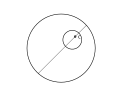
\includegraphics[width=0.35\textwidth]{hyperbolicCircle}
    \caption{An example of a hyperbolic circle not centered at the origin}
    \label{fig:hyperbolicCircle}
  \end{figure}


\section*{Parabolas}
In the previous section, we analyzed the images of circles under a variety of distance functions. This was possible as the equation of a circle can be written in terms of distances. Given this process, we can now consider the image of other shapes so long as they are given in terms of distances. Another common shape that arises in from the discussion of conic sections is the parabola. Typically, we identify a parabola as a function of the form
\begin{equation*}
  f(x) = A(x-H)^^2+K
\end{equation*}
which has a single vertex at the point $(H,K)$. There is a second way to define the parabola solely in terms of distances.

\definition{A \textbf{parabola} is a curve such that every point is equidistant to a point called the focus and a line called the directrix}


\begin{figure}[!hbt]
  \centering
  \includegraphics[width=0.5\textwidth]{directrix}
  \caption{Diagram of the distance definition of a parabola \cite{parabola}}
  \label{fig:directrix}
\end{figure}

Thus with this definition, we can see how the image of the standard parabola shown in figure \ref{fig:directrix} changes as we change the distance function. If we allow $d$ to be a general distance function, then this definition can be spelled out as follows. Consider the line $\ell(x) = (x,c)$ for some constant $c$. Also, consider a point $f=(f_x, f_y)$ which will be the focus of the parabola. Then the parabola defined by the directrix $\ell$ and the focus $f$ is given by
\begin{equation*}
  P = \left\{(x,y) \in\R^2\Big| d\big((x,c),(x,y)\big)-d\big((f_x,f_y),(x,y)\big)=0   \right\}
\end{equation*}

Given this definition for the parabola, let's examine some examples for the various distance functions. I will solve for the curve by numerically solving for points satisfying the above definition for $c = 0$ and $f_x=0, f_y = 2$.  

\begin{figure}[!hbt]
  \hspace{-3em}
  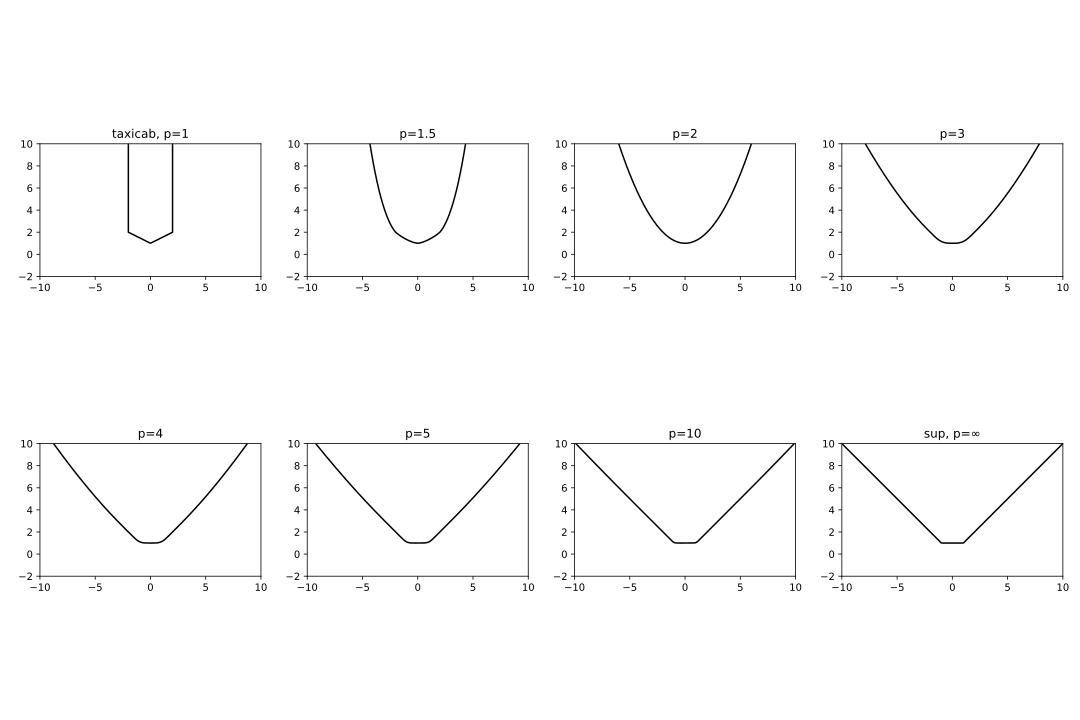
\includegraphics[width=1.15\columnwidth]{parabolas}
  \caption{Parabolas under different distance functions} 
\end{figure}

It is interesting to note how the behavior here is similar to when we plotted the circles. When $p=2$ we have our standard straight line distance and so the resulting parabola has the familiar shape. As we decrease and increase $p$ beyond this point, we see that the resulting image becomes less and less smooth.

\section*{Conclusions}
We have defined the concept of the distance function and illustrated its value in geometric proofs where the geometric properties we care about involve length. We then examined the images of two common figures, the circle and the parabola, under these different distance functions. It is very interesting to note how the shape of the images moves away from being smooth for the generalized Euclidean distance and towards images that are notably not smooth when $p$ goes away from the value of 2.

Given more time I would like to explore the images of other figures that can be defined in terms of distance. A follow up topic could also examine the consequence of changing the Euclidean $p=2$ distance in the affine, projective, and inversive geometries. This could be particularly interesting for inversive geometry where we define the inversion in a circle with radius $r$ and center $\mathcal{O}$ as sending the point $A$ to $A'$ such that
\begin{equation*}
    d(\mathcal{O}, A)\cdot d(\mathcal{O}, A') = r^2
\end{equation*}

\noindent I would be curious to see how the transformations of lines and circles are different under such a change.




\bibliography{references}
\bibliographystyle{ieeetr}

\end{document}




















